% -----------------------------------------------------------------------------

\begin{frame}{Demographics - Pi charts}
    \begin{columns}[c] % The "c" option specifies centered vertical alignment while the "t" option is used for top vertical alignment

        \column{.5\textwidth} % Right column and width
    
        \begin{figure}
        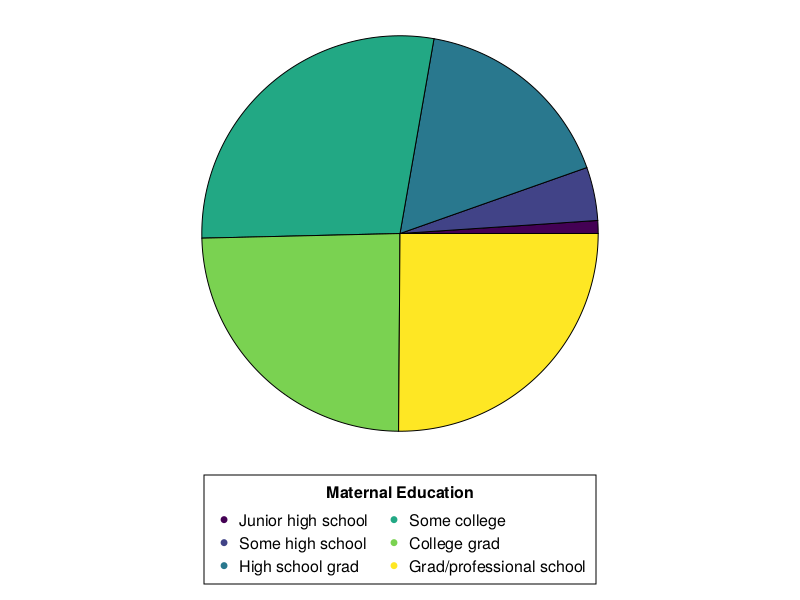
\includegraphics[width=1\linewidth]{../figures/demo_education.png}
        \end{figure}

        \column{.5\textwidth} % Right column and width
    
        \begin{figure}
        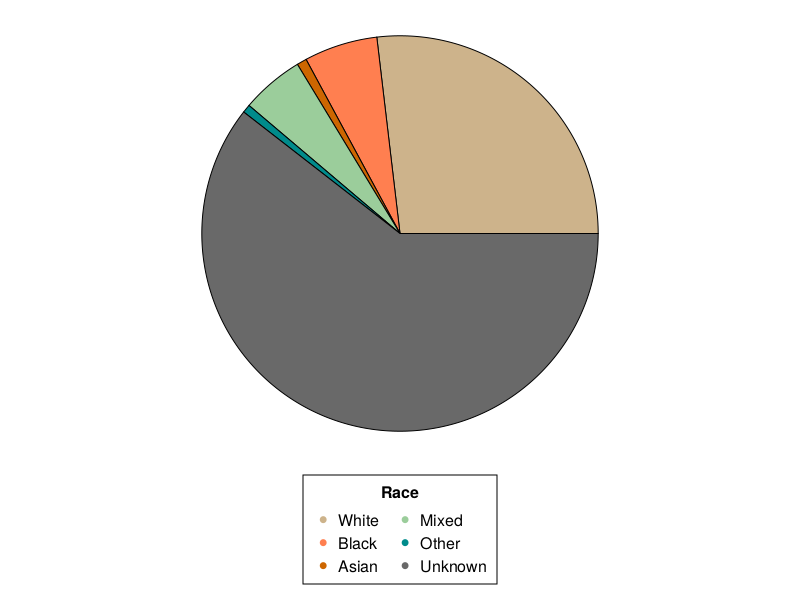
\includegraphics[width=1\linewidth]{../figures/demo_race.png}
        \end{figure}

    \end{columns}

    \textbf{Details}
    \begin{enumerate}
        \item Education does not include missings
        \item Race numbers not from database, using counts from RI group
    \end{enumerate}

\end{frame}

% -----------------------------------------------------------------------------

